\Section{Data Sources} 

The type of data being compressed plays an important factor in how
well a compression algorithm will do.  Certain types of data will
favor one compression scheme over another compression scheme.  We
evaluate several compression schemes on three types of sensor data
collected from actual sensor network deployments.  

\subsection{Seismic Volcano Data}

We look at seismic data from a 19-day sensor network deployment at
Revenatador~\cite{volcano-osdi06}, an active volcano in Ecuador in
August of 2005.  Active volcanos produce many small earthquakes
throughout the day.  Monitoring and localizing these earthquakes allow
the volcanologists studying the volcano to make better predictions
about future eruptions from the volcano.  Telos motes were used to
collect seismic data from these earthquakes with a custom ADC sampling
board attached to the motes.  The seismic data was sampled at 100 Hz
and captured with 24 bits of resolution.  We looked at 229 earthquakes
over the 19 day period.  A sample of the data is shown in
Figure~\ref{volcano-data}.

\begin{figure}[h]
  \centering
  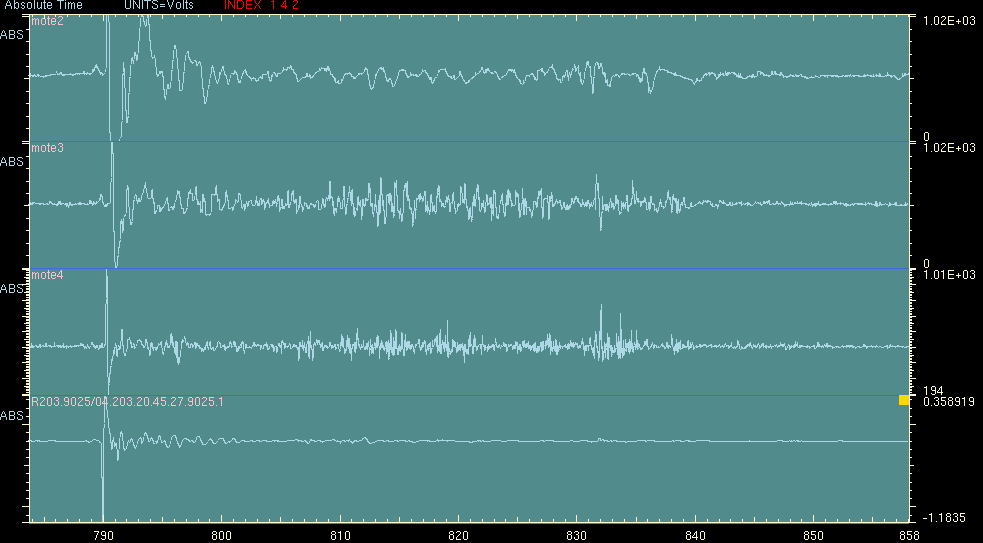
\includegraphics[width=0.5\textwidth]{figures/volcano-data.png} 
  \caption{Seismic data for four nodes at the start of an earthquake.}
  \label{fig:volcano-data}
\end{figure}

\subsection{Acoustic Data for Wildlife Habitat Tracking}

\subsection{Body Sensor Network Data}
